\begin{figure}
    \centering
\begin{knitrout}
\definecolor{shadecolor}{rgb}{0.969, 0.969, 0.969}\color{fgcolor}
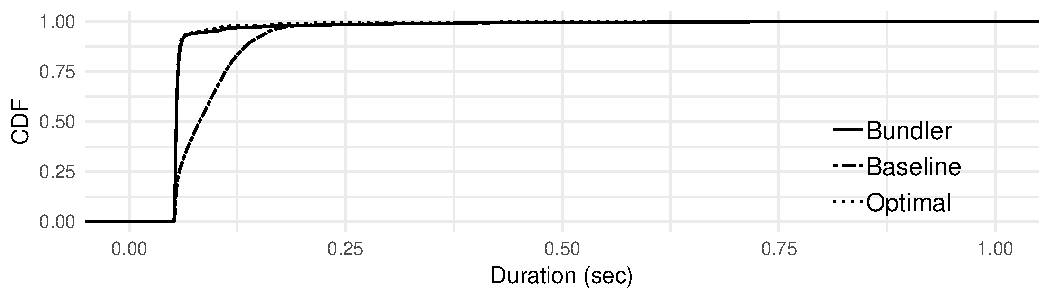
\includegraphics[width=\maxwidth]{figure/eval:best-1} 

\end{knitrout}
    \caption{\name achieves 28\% lower median slowdown. 
The three graphs show FCT distributions for the indicated request sizes: smaller than 10KB, between 10KB and 1MB, and greater than 1MB.  Note the different y-axis scales for each group of request sizes. Whiskers show $1.25 \times$ the inter-quartile range. 
For both \name and Optimal, performance benefits come from preventing short flows from queueing behind long ones. 
Thus, \name's aggregate congestion control by itself is not enough; if we configure \name to use FIFO scheduling, the FCTs worsen compared to the status quo.
    \fc{Status quo whiskers are too large to fit on plot, mention the number here.}}
    \label{fig:eval:best}
\end{figure}
\newcommand{\overviewBenefitsBaselineMedian}{1.76\xspace}
\newcommand{\overviewBenefitsBaselineTail}{79.37\xspace}
\newcommand{\overviewBenefitsBundlerMedian}{1.26\xspace}
\newcommand{\overviewBenefitsBundlerTail}{41.38\xspace}
\newcommand{\overviewBenefitsOptimalMedian}{1.07\xspace}
\newcommand{\overviewBenefitsOptimalTail}{27.49\xspace}
\newcommand{\overviewBenefitsBundlerMedianImprovement}{28\%\xspace}
